\chapter{実験}
\label{experiment}
%仮説を検証するためにやったことを再現可能な様に書く
%結果も書く

本章では提案手法の実装について述べる。

\section{概要}
\label{sub:実験概要}
本研究の仮説をもとに、システムの実装をおこなった。
\begin{figure}[h]
  \begin{center}
      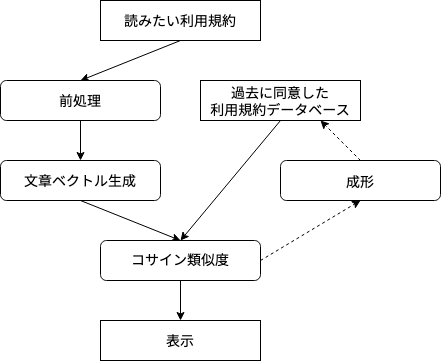
\includegraphics[width=10cm]{img/system.drawio.png}
      \caption{類似条文検出の実装イメージ}
      \label{img:類似条文検出の実装イメージ}
  \end{center}
\end{figure}

\section{表示方法}
表示方法については、利用規約の類似条文検出に加えて、判断の材料にするために、類似度の高い順に3つの条文とその条文をもつサービス名、コサイン類似度を表示した。3つに設定した根拠としては、他サービスの条文と比較するときに複数サービスの条文と比較することで、より類似度を利用者が比較しやすいと考えたからである。

%\section{実行環境}
%\begin{center}
%  \begin{tabular}{ll} \hline
%    項目 & 仕様 \\ \hline \hline
%    環境 & Azure Web App Service\\
%    インスタンス & B1 \\
%    コア数 & 1 \\
%    RAM & 1.75GB \\ \hline
%  \end{tabular}
% \end{center}

%%% Local Variables:
%%% mode: japanese-latex
%%% TeX-master: "../bthesis"
%%% End:
